\documentclass{article}
\usepackage{graphicx} % Required for inserting images
\usepackage{amsmath}
\usepackage{booktabs}
\usepackage{array}
\usepackage{enumitem}
\usepackage{xcolor}
\usepackage{titlesec}
\usepackage{fancyhdr}
\usepackage{listings}
\title{Introduction to Distributed Systems}
\author{0xSaad}
\date{October 2026}

\begin{document}

\maketitle

\section{Centralized Computing}

Early form of computing was centralized , Also called Uniprocessor computing.

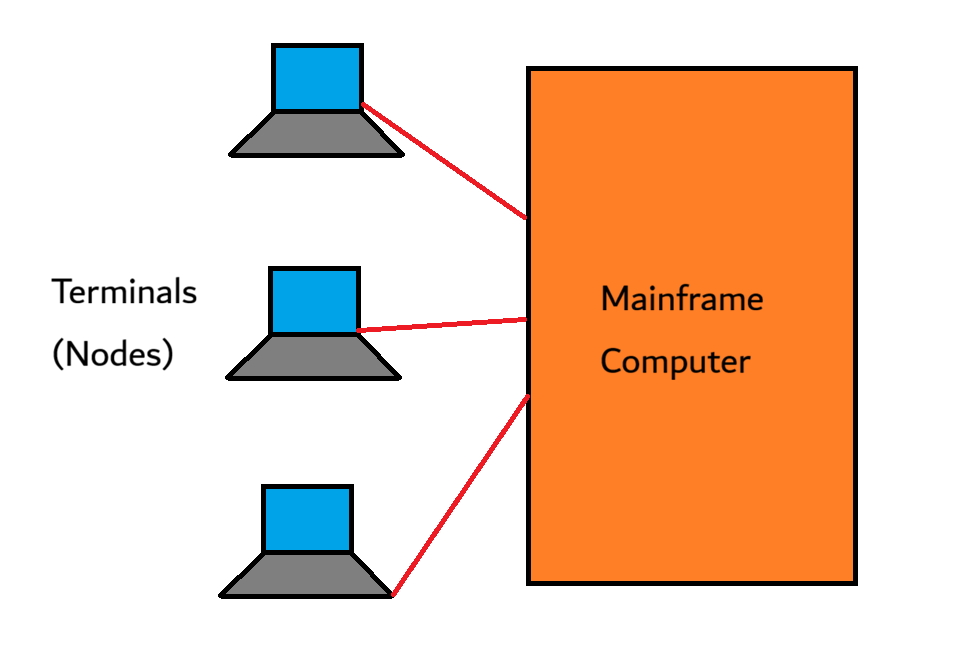
\includegraphics[width=0.5\textwidth]{images/centralized.png} \\

\section{What is distributed system ?}

Collection of independent computers interconnected via network collaborating on tasks

\subsection{Another declaration}

Collection of autonomous computing elements that appears to users as Single coherent system

Each node is autonomous and have it's own notion of time , there is no global clock.

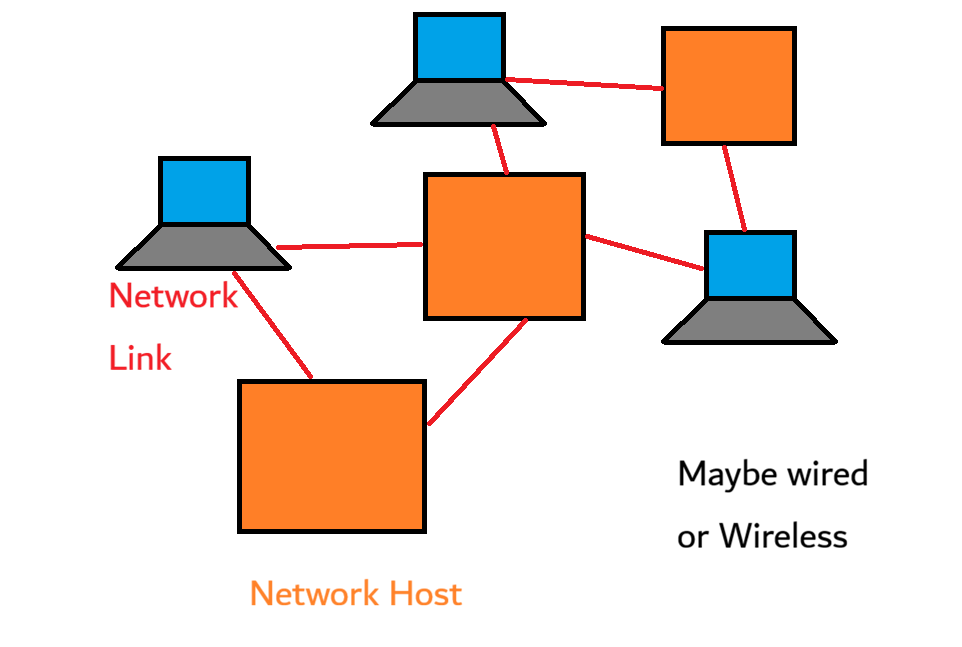
\includegraphics[width=0.5\textwidth]{images/distributed.png} \\


\section{Coherent system}

The nodes in system as whole operates the same.

No matters where or when or how users and system interaction takes a place.

\section{Overlay Network}
Logical network which each node communicates with set of others node called \textbf{neighbors}.

P2P Systems is good example for overlay networks

\subsection{Types of overlay networks}
\begin{itemize}
    \item Structured : Well-defined set of neighbors
    \item Unstructured : Randomly selected neighbors
\end{itemize}

\section{Computers in Distributed Systems}
\begin{itemize}
    \item Workstations : Used by End-users to perform computing
    \item Servers : Provides services and resources
    \item PADs (Personal Assistance Devices)
\end{itemize}

\subsection{Examples of Distributed Systems}
\begin{itemize}
    \item Internet
    \item ATM Machines
    \item Intranets / Workgroups
\end{itemize}

\subsection{Types of Distribution Systems}
\begin{itemize}
    \item High performance distributed systems (Parallel - Grid - Cluster - Cloud)
    \item Distributed Information Systems (Middleware-EAI-TPM)
    \item Distributed systems for pervasive computing (Ubitiqouis - Mobile - Sensor networks)

\end{itemize}

\section{Characteristics of Distributed Systems}
\begin{enumerate}
    \item Heterogeneity are mostly hidden
    \item Users interact consistently and uniformly with system
    \item Easy to expand or scale
    \item It's normally continuous avaliable
\end{enumerate}

\section{Main goals of Distributed Systems}
\begin{itemize}
    \item Sharing of resources and services
    \item Distribution Transparency
    \item Openness
    \item Scalability
\end{itemize}

\subsection{Scalability}

Be Able to add more users and devices to system

And be able to separate users and devices geographically.

\subsubsection{Scaling Techniques}

\begin{itemize}
    \item Hiding communication latencies
    \item Distribution which splitting it into smaller parts and subsequently spreading
    \item Replication components across a distributed system
\end{itemize}


\section{Challenges of Distributed Systems}
\begin{itemize}
    \item Heterogeneity (2 Kinds of OS)
    \item Latency
    \item Synchronization
    \item DoS Attacks
    \item Partial Failure
\end{itemize}
\end{document}
